\section{Numerical Examples}
\label{sec:ex}

In this section, we showcase GAIL's performance with two examples on
univariate function optimization and cubature.

\begin{example}\label{eg1} We want to find the global minimum of the following functions: 
\begin{align}
    f(x) &= -5 \E^{-100(x-0.15)^2}-\E^{ -80(x-0.65)^2}  \mbox{ for } x \in [0, 1], \label{eq1}
\\  f(x) &= \sin (10 \pi x^4 ) - x  \mbox{ for } x \in [0, 2]. \label{eq2}
\end{align}
In the case of (\ref{eq1}), \texttt{funmin\_g} automatically samples the
function more often in spiky areas and locates the global minimum
accurately. In contrast, MATLAB's
\texttt{fminbnd}~\cite{brent2013algorithms,forsythe1977computer} returns a
local minimum.  That said, we note that \texttt{fminbnd} was designed for
seeking a local minimum. Chebfun~\cite{TrefEtal17a} approximates $f$ with
Chebyshev polynomials and samples $f$ at Chebyshev points. Its \texttt{min} function is 
capable of returning all local minimum that it
could find, out of which we extract the global minimum. Both \texttt{min} and
\texttt{funmin\_g} succeeded in locating the global minimum to required
accuracy, with the former being more efficient with fewer sampling points
and the latter more accurate.


In the case of (\ref{eq2}), we have a function that is increasingly
oscillating as $x$ increases and the true minimum occurs at the right
boundary point. Both \texttt{min} and \texttt{funmin\_g} were able to return  
accurate approximations, but \texttt{fminbnd} once again settled at a local
minimum far away from the global minimum. The total run time of
\texttt{funmin\_g} was substantially less than that of \texttt{min} because it
sought only the global minimum and disregarded the other local minima.

We plot $f(x)$ and the minima returned by \texttt{funmin\_g}, \texttt{min},
and \texttt{fminbnd}  for the two given functions in Figures~\ref{fig1} and
\ref{fig2}. In addition, Table~\ref{tab1} summarizes the solvers'
performance.

\begin{figure} % MATLAB Driver: min_pearc.m
\centering
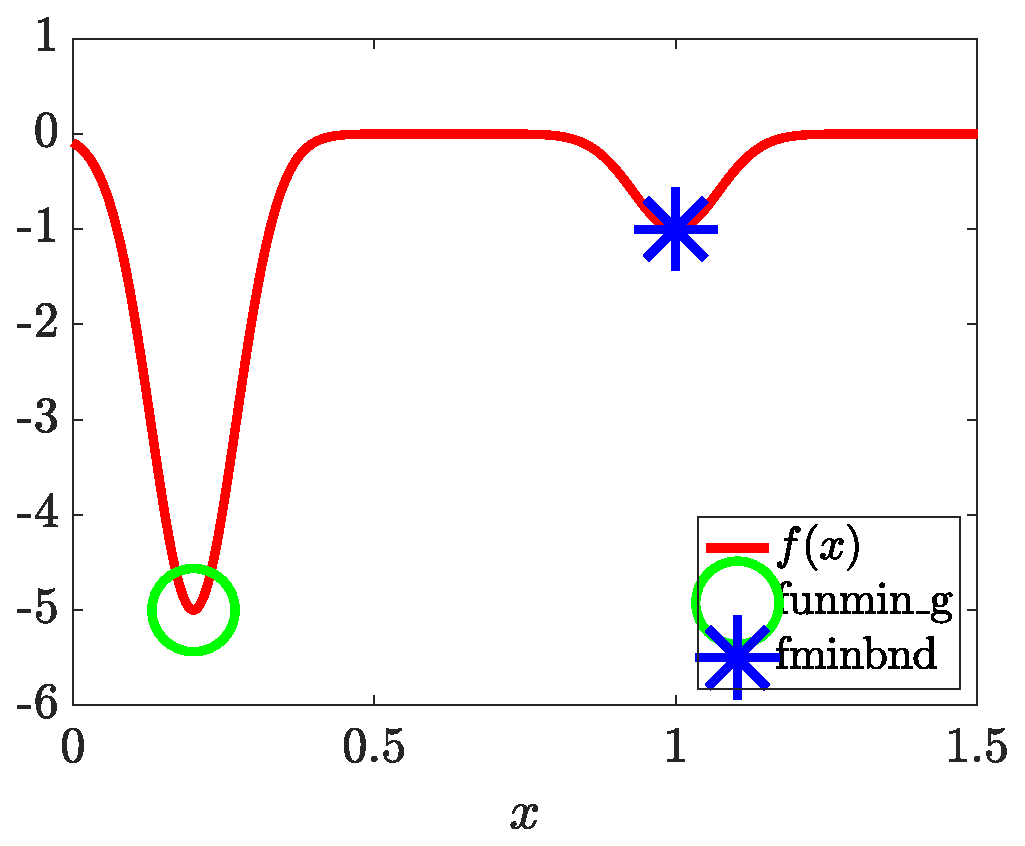
\includegraphics[width = 0.48\textwidth]{humps.eps} 
\caption{We plot the function $f$ in (\ref{eq1}), along with the sampling
points and best estimates of $(x^*, f(x^*)$ from the three solvers,
MATLAB's \texttt{fminbnd}, Chebfun's \texttt{min}, and GAIL's \texttt{funmin\_g}. 
This figure is
reproducible by the MATLAB script, \texttt{min\_pearc.m}, in GAIL.}\label{fig1}
\end{figure}

\begin{figure} % MATLAB Driver: min_pearc.m
\centering
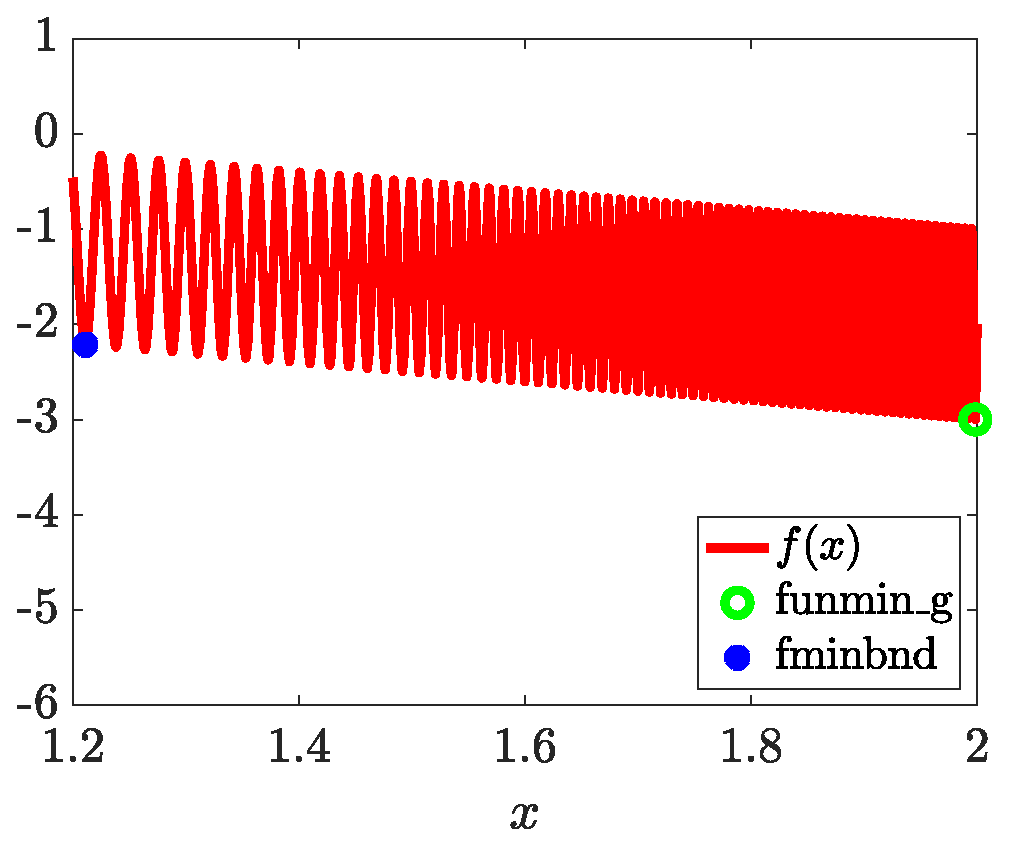
\includegraphics[width = 0.48\textwidth]{sine.eps} 
\caption{
This figure is reproducible by the script, \texttt{min\_pearc.m}, in GAIL.}\label{fig2}
\end{figure}

\begin{table} % MATLAB Driver:  min_pearc.m
\centering
	\caption{Performance of \texttt{funmin\_g}, \texttt{fminbnd}, and
	\texttt{min} with automatic stopping criteria for optimizing
	functions defined in (\ref{eq1}) and (\ref{eq2}). Absolute errors in
	$x$  and $y$ are defined as $|x^* - \hat{x}|$ and $|f(x^* ) -
	f(\hat{x})|$, respectively. These results can be reproduced with script
	\texttt{min\_pearc.m} in GAIL. \label{tab1}}  \vspace{-2ex}
	$
    \begin{array}{l@{\qquad}r@{\quad}r@{\quad}r}
	\input{minPearcOut.txt} 
	\end{array}
	$
\end{table}
\end{example}


\begin{example}\label{eg4}  
In this example, we compare GAIL's Monte Carlo and quasi-Monte Carlo
methods in similar ways as in Section~4 in \cite{hickernellmonte} with the
Keister integrals~\cite{keister1996multidimensional}:
\begin{align}
\mu % & =  \int_{\R^d} \cos(\lVert \vt \rVert_2)  \E^{-\lVert\vt \rVert_2^2} \, \dif \vt \\
& = \bigint_{[0,1]^d} \pi^{d/2} 
\cos \left( \sqrt{ \frac{1}{2} \sum_{j=1}^d \Phi^{-1}(x_j)} \right)  \, \dif \vx. 
\label{kei}
\end{align}

In Table~\ref{tab2}, we summarize the performance of the methods MC, Sobol,
 Lattice, and Bayes---they refer to the GAIL cubatures, \texttt{cubMC\_g},
\texttt{cubLattice\_g}, \texttt{cubSobol\_g},  \texttt{cubBayesLattice\_g},
respectively.
In the case of $d=3$, all four methods succeeded completely meaning the
absolute error is less than given tolerance, i.e., $|\mu - \hat{\mu}| \le
\varepsilon$, where $\hat{\mu}$ is a cubature's approximated value. The
fastest method was \texttt{cubBayesLattice\_g}.
In the case of $d=8$,   \texttt{cubSobol\_g} achieved 100\% success rate
and was the fastest. But \texttt{cubBayesLattice\_g}  was competitive and
had the smallest average absolute error.

\begin{table} % MATLAB Driver: KeisterCubatureExamplePEARC.m
\centering
	\caption{Average performance of cubatures with automatic stopping 
	criteria for estimating the integrals in \eqref{kei}
	for $1000$ independent runs. These results can be conditionally reproduced with the
	script, \texttt{KeisterCubatureExamplePEARC.m}, in GAIL. 
	\label{tab2}}	   \vspace{-2ex}
	$
	%\arraycolsep=1.4pt\def\arraystretch{0.9}
    \begin{array}{l@{\qquad}r@{\quad}r@{\quad}r@{\quad}r@{\quad}r}
	\input{KeisterPearcOut.txt} 
	\end{array}
	$
\end{table}


\end{example} 